% Style taken from http://www.ctan.org/tex-archive/info/MemoirChapStyles/MemoirChapStyles.pdf
\documentclass[oldfontcommands,openany,oneside]{memoir}
\chapterstyle{dash}
\usepackage{graphicx}
\usepackage{amsmath}
\usepackage{latexsym}
\usepackage{units}
\usepackage{mathrsfs}
\usepackage{pdflscape}
\usepackage{courier}
\usepackage{placeins}
\usepackage[breaklinks=true, hidelinks]{hyperref}
\usepackage{framed}
\usepackage{color}
\usepackage{menukeys} % e.g. \keys{\shift + F} see: https://tex.stackexchange.com/questions/5226/keyboard-font-for-latex
\usepackage{tcolorbox} % For nice boxes!
\usepackage{fontawesome} % For the folder and file symbal used in \file and \dir.

\usepackage{dirtree}
\renewcommand*\DTstylecomment{\rmfamily\color{red}\small}
%\renewcommand*\DTstyle{\ttfamily\textcolor{red}} % remove the comment to change the color to red


\pretitle{\begin{center}\LARGE\sffamily}
\posttitle{\par\end{center}\vskip 0.5em}
\predate{\begin{flushright}\large\scshape}
\postdate{\par\end{flushright}}

%Authors, title, Journal, vol, page, year, doi
\newcommand{\myref}[7]{\href{http://dx.doi.org/#7}{#1 -- \emph{#2.}\\ #3 \textbf{#4}, #5 (#6)}.}
\newcommand{\note}[1]{\paragraph{Note}#1}
\newcommand{\red}[1]{\textcolor{red}{#1}}

\newcommand{\file}[1]{{\fontsize{9}{0}\selectfont\faFileTextO}$\,${\fontsize{7}{0}\selectfont\faCaretRight}\directory{#1}}
\newcommand{\dir}[1]{{\fontsize{9}{0}\selectfont\faFolderOpen}$\,${\fontsize{7}{0}\selectfont\faCaretRight}\directory{#1}}
\newcommand{\dird}[1]{{\fontsize{9}{0}\selectfont\faFolderOpen}$\,${\fontsize{7}{0}\selectfont\faCaretDown}\directory{#1}}
\newcommand{\dirclosed}[1]{{\fontsize{9}{0}\selectfont\faFolder}$\,${\fontsize{7}{0}\selectfont\faCaretRight}\directory{#1}}

\newcommand{\dirTorri}[1]{{\fontsize{9}{0}\selectfont\faFolderOpenO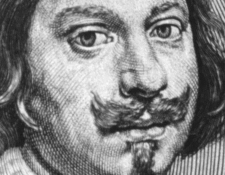
\includegraphics{img/Torricelli_icon.png}}$\,${\fontsize{7}{0}\selectfont\faCaretRight}\directory{#1}}
\newcommand{\dirData}[1]{{\fontsize{9}{0}\selectfont\faFolderOpenO$\mathcal{D}$}$\,${\fontsize{7}{0}\selectfont\faCaretRight}\directory{#1}}

\newcommand{\fileTorri}[1]{{\fontsize{9}{0}\selectfont\faFileO\hspace{1px}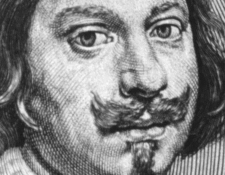
\includegraphics{img/Torricelli_icon.png}}$\,${\fontsize{7}{0}\selectfont\faCaretRight}\directory{#1}}
\newcommand{\fileData}[1]{{\fontsize{9}{0}\selectfont\faFileO$\mathcal{D}$}$\,${\fontsize{7}{0}\selectfont\faCaretRight}\directory{#1}}

\title{\textsc{Torricelli}: A software to determine atomic spatial distribution from normal incidence x-ray standing wave data\\  {\large -- \emph{Manual of version 3.8} --\\ \vspace{.5cm} \begin{framed} See Ref.~\cite{Bocquet2018} for a review of the used theory and approximations.\\  \vspace{.5cm} The latest updates are available on \textcolor{blue}{\href{www.torricelli-software.com}{www.torricelli-software.com}}. \end{framed}}}
\author{\vspace{5cm}F. C. Bocquet, G. Mercurio and M. Franke}
\date{\today}

\begin{document}
\frontmatter
\maketitle
\begin{center}
  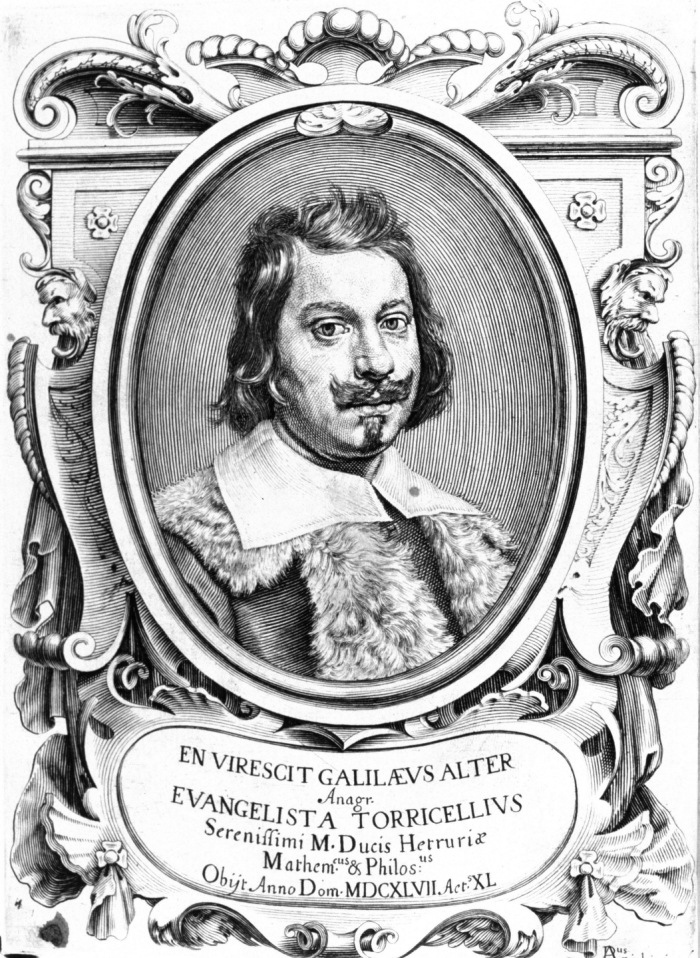
\includegraphics{img/Torricelli_Portrait.jpg}\\
  {\tiny(Image in the Public Domain)}
\end{center}




%%%%%%%%%%%%%%%%%%%%%%%%%%%%%%%%%%%%%%%%%%%%%%%%%%%%%%%%%%%%%%%%%%%%%%%%%%%
\chapter{Preface}
 \textsc{Torricelli} is a software designed for the analysis of x-ray standing wave (XSW) data. While the XSW technique has been employed for several decades, to our knowledge no free, open source, user-friendly and well-documented program for conducting XSW data analysis exists to date. \textsc{Torricelli} is therefore an attempt to fill this gap. The spatial distribution of atomic species with respect to  the atomic planes of a single crystal can be described by two parameters, the coherent position $P_\mathrm{c}$ and the coherent fraction $F_\mathrm{c}$. The main target of \textsc{Torricelli} is to determine this pair of parameters in the most accurate way, and also provide the corresponding statistical errors \cite{Mercurio2013, Bocquet2018}.\\

We encourage the readers to make suggestions that could improve the program as well as the present manual. If you can program in python you are also welcome to take part in the programming. \textsc{Torricelli} is distributed under the GNU General Public License v3. You should have received a copy of the GNU General Public License along with \textsc{Torricelli}.  If not, see \url{https://www.gnu.org/licenses}. This manual is distributed under the creative commons Attribution-ShareAlike license (CC BY-SA 4.0), see \url{https://creativecommons.org/licenses/by-sa/4.0/legalcode}.\\

We would like to thank particularly Tien-Lin Lee for discussing the fitting equations and their implementation. Of course, all the \textsc{Torricelli} users are also thanked for reporting small bugs, and encouraging development. \newpage

\tableofcontents
\mainmatter

%%%%%%%%%%%%%%%%%%%%%%%%%%%%%%%%%%%%%%%%%%%%%%%%%%%%%%%%%%%%%%%%%%%%%%%%%%%
\chapter{Getting started}
\chaptermark{Getting started} % for the header
\section{Installation} %%%*********************************%%%
\textsc{Torricelli} is an interpreted program. That means first you need to install Python and a few modules in order to be able to launch \textsc{Torricelli} (which itself does not require any installation). \textsc{Torricelli} was programmed in \texttt{Python2.7} and \texttt{PyQt4}. Compatibility to \texttt{Python3} and/or \texttt{PyQt5} is not supported at the moment. If you already have a scientific \texttt{Python2.7} installation, you can test your installation by trying to import the following packages in a python console:

\begin{verbatim}
>>> import scipy, numpy, cmath, lmfit
>>> import pyqtgraph
>>> from pyqtgraph.Qt import QtGui, QtCore
>>> from PyQt4.QtCore import pyqtSignal, pyqtSlot
>>> from PyQt4 import QtCore, QtGui
>>> import ConfigParser, csv, sip, colorsys
>>> import sys, string, os, datetime, glob, ast
>>> from distutils.version import StrictVersion
>>> from operator import itemgetter
\end{verbatim}

That will load one by one all the necessary modules required by \textsc{Torricelli}. \emph{None} of these lines should return \emph{any} error message. If it does, that means there are missing packages that should be installed, as explained in the following. You may see a 'FutureWarning' message depending on the version you use. Also there is a small bug in one of the packages that is needed to run Torricelli. There is a workaround explained after the installation instructions.

\subsection{Linux}
Simply install the following packages with your preferred package manager: \verb+Pyhton2.7+,  \verb+PyQt4+,  \verb+pyqtgraph+, \verb+numpy+, \verb+scipy+, and \verb+lmfit+

\paragraph{Note} Once \verb+Pyhton2.7+ is installed, you can also use \verb+pip+ to install the rest (useful to get the latest \verb+pyqtgraph+ version on some distributions). 

\subsection{Windows}
We recommend to install the package manager \verb+Miniconda+  for \verb+Python 2.7+ (\href{https://conda.io/miniconda.html}{https://conda.io/miniconda.html}). During the installation, check the box \emph{add Anaconda to the PATH} (if not, you will have to use the anaconda prompt for Torricelli, which is fine but less practical). After installation, execute the following commands:
\begin{itemize}
\item \texttt{conda install pyqt=4 numpy scipy}
\item \texttt{pip install lmfit pyqtgraph}
\end{itemize}

\subsection{Mac}
We recommand to install the package manager \texttt{Homebrew} (\href{https://brew.sh}{https://brew.sh}). After installation, execute the following commands in a console:
\begin{itemize}
\item \texttt{brew install python}
\item \texttt{sudo easy\_install pip} (may not be necessary with the latest homebrew version)
\item \texttt{pip install pyqt numpy scipy lmfit pyqtgraph}
\end{itemize}

\paragraph{Small bug} There is a tiny bug in the latest version of pyqtgraph (0.10.0). The problematic line number and file name will display in the console (\texttt{ImageExporter.py} at line 70) when you use Torricelli. A couple of \textcolor{red}{\textttt{\bf int()}} must be added:\\
\verb+bg = np.empty((+\textcolor{red}{\textttt{\bf int(}}\verb+self.params['width']+\textcolor{red}{\textttt{\bf )}},\\
\verb+               + \textcolor{red}{\textttt{\bf int(}}\verb+self.params['height']+\textcolor{red}{\textttt{\bf )}}\verb+, 4), dtype=np.ubyte)+\\
You will find the file in the directory \verb+...\pyqtgraph\exporters+ in your site-packages directory. If you do not know where your site-package folder is, type\\
\verb+import site; site.getsitepackages()+ in the python console and it will be displayed.

\subsection{Upgrading packages}
To upgrade any of the packages, one can simply run the following command:
\verb+conda update <package_name>+\\
or\\
\verb+pip install <package_name> -U+\\
depending on how you installed the package.



\section{Conventions used in this manual}
\begin{itemize}
\item \dirTorri{Here/folder}: designates the sub-path in the folder containing the \textsc{Torricelli} program.
\item \fileTorri{Here/the/file.txt}: designates a file in a sub-folder of the \textsc{Torricelli} program.
\item \dirData{Some/folder}: designates the sub-path in the folder containing the data to be analyzed.
\item \fileData{All/data1.dat}: designates a file in a sub-folder of the folder containing the data to be analyzed.
\item The coming references in bracket, like ($n$), indicate fields or buttons marked in the region of interest of the program screenshot shown in the figures.
\end{itemize}

\section{Launching \textsc{Torricelli}} %%%*********************************%%%

There are several possibilities to  start \textsc{Torricelli}.
\begin{itemize}
\item[\textcolor{green}{$\bullet$}] We recommend to open a console, change directory (command \texttt{cd} on Linux, Mac and Windows) to the program folder (\dirTorri{}) and execute \verb+python Torricelli.py+.
\item[\textcolor{green}{$\bullet$}] One also can double click on the file \fileTorri{\textsc{Torricelli}.py} if it is executable on your system. 
\item[\textcolor{red}{$\bullet$}] Do not start \textsc{Torricelli} from an interactive python shell.
\end{itemize}
Before starting an analysis, one must first define the directory that contains your experimental files (\dirData{}) (1), by clicking on the \keys{...} button (2). In this folder, a \dirData{results/} sub-folder is created and will contain all results (as ASCII files and pictures).

\begin{figure}[!h]
  \centering
  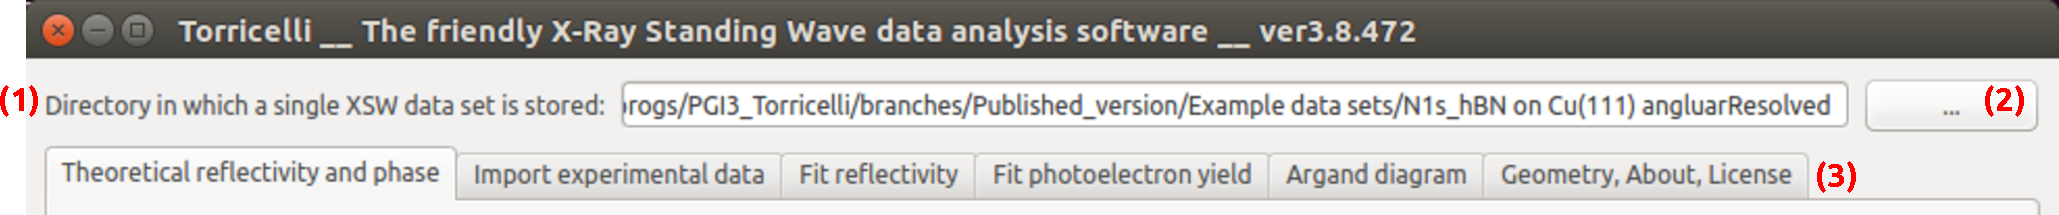
\includegraphics[width=1\textwidth]{img/Screenshot_Tab.pdf}
  \caption{The tab structure of \textsc{Torricelli}.}
  \label{fig:Tab}
\end{figure}

  \textsc{Torricelli} is organized in tabs (3) (Fig.~\ref{fig:Tab}). There is a separate tab for each important step of the data analysis. One can scroll from tab to tab with the mouse wheel, or using the shortcuts \keys{Ctrl+PageUp} and \keys{Ctrl+PageDown}. In this manual, a chapter is dedicated to each tab necessary to the data analysis. The details of the algorithm are described in Ref.~\cite{Bocquet2018} and should be read together with this manual.

We tried to add as much information as possible in 'tooltips', see Fig. \ref{fig:tooltip}. Rest the mouse cursor on a given object for one second, and a box will appear with some explanations if there is anything to clarify.

\begin{figure}[!h]
  \centering
  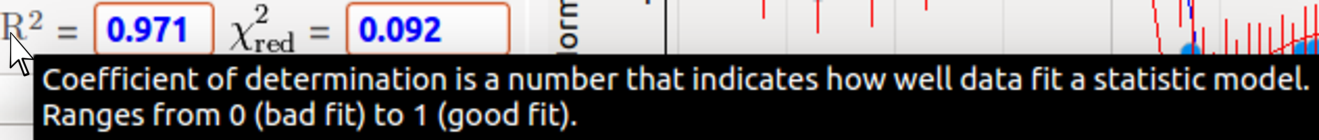
\includegraphics[width=\textwidth]{img/Screenshot_Tooltip.pdf}
  \caption{Example of a tooltip on $R^2$.}
  \label{fig:tooltip}
\end{figure}

%%%%%%%%%%%%%%%%%%%%%%%%%%%%%%%%%%%%%%%%%%%%%%%%%%%%%%%%%%%%%%%%%%%%%%%%%%%
\chapter{Theoretical reflectivity and phase} \label{chap:structureFactor}
The calculation of the structure factors requires the knowledge of the (sample and monochromator) crystallographic parameters: lattice constants, and list of atoms in the unit cell. Besides, the Debye-Waller factor can also be added if known. 

There exist two databases of crystallographic parameters, for elemental (\file{CrystallographicData\_Elemental.csv}) and for compound (\file{Cry\\stallographicData\_Compound.csv}) samples. They can be found in the folder \dirTorri{imports/Databases/Lattices/}. Each crystal has a dedicated line, with comma separated values, e.g.,
\begin{center}
  \fbox{\begin{minipage}{\textwidth}
      \fileTorri{imports/Databases/Lattices/CrystallographicData\_\\Elemental.csv}\\
      Contains the lattice constants of all elemental crystal:
        \hline \\\vspace{10pt}
      Z,Name,cell\_type,a,b,c,alpha,beta,gamma,checked\_values\\
      14,Si,diamond,543.09,543.09,543.09,90,90,90,yes\\
      28,Ni,faceCentered,352.4,352.4,352.4,90,90,90,no\\
      29,Cu,faceCentered,361.49,361.49,361.49,90,90,90,yes\\
      $\vdots$
  \end{minipage}}
\end{center}
First comes the atomic number of the atom(s), the element name, the type of unit cell, the three lattice lengths ($a,b,c$) in [pm], the three lattice angles ($\alpha, \beta, \gamma$) in [$^\circ$]. The last argument (checked\_values) specifies if the values has already been used in the analysis of NIXSW data. This is then displayed in the graphical user interface to draw the user's attention on crystallographic parameters that were taken from various references but not tested (see file \fileTorri{imports/Databases/Database references.txt} for the sources). If your sample has a complex unit cell that is not in the database, you can create a file named \fileTorri{imports/Databases/Lattices/AtomCoordinates\_\\name-of-unit-cell.csv} that lists the relative position of all atoms. For example, for the face-centered unit cell we have:
\begin{center}
  \fbox{\begin{minipage}{\textwidth}
      \fileTorri{imports/Databases/Lattices/AtomCoordinates\_\\faceCentered.csv}\\
      Atomic positions in the face centered unit cell:
        \hline \\\vspace{10pt}
      Element,x (a),y (b),z (c)\\
      A,0,0,0\\
      A,.5,.5,0\\
      A,.5,0,.5\\
      A,0,.5,.5
  \end{minipage}}
\end{center}
Then just add a line in the \fileTorri{imports/Databases/Lattices/Crystallo\\graphicData\_*.csv} file that indicates \texttt{name-of-unit-cell} in the column \texttt{cell\_type} as well as the atomic mass and the crystal parameters. After restarting \textsc{Torricelli}, the new crystal will be included in the database.

\paragraph{Note} If you successfully used not-checked-yet values in experiments, or included new samples/unit cells into the database, please contact the developers to include your values to the next version of \textsc{Torricelli}.\\\\

\begin{figure}[!b]
  \centering
  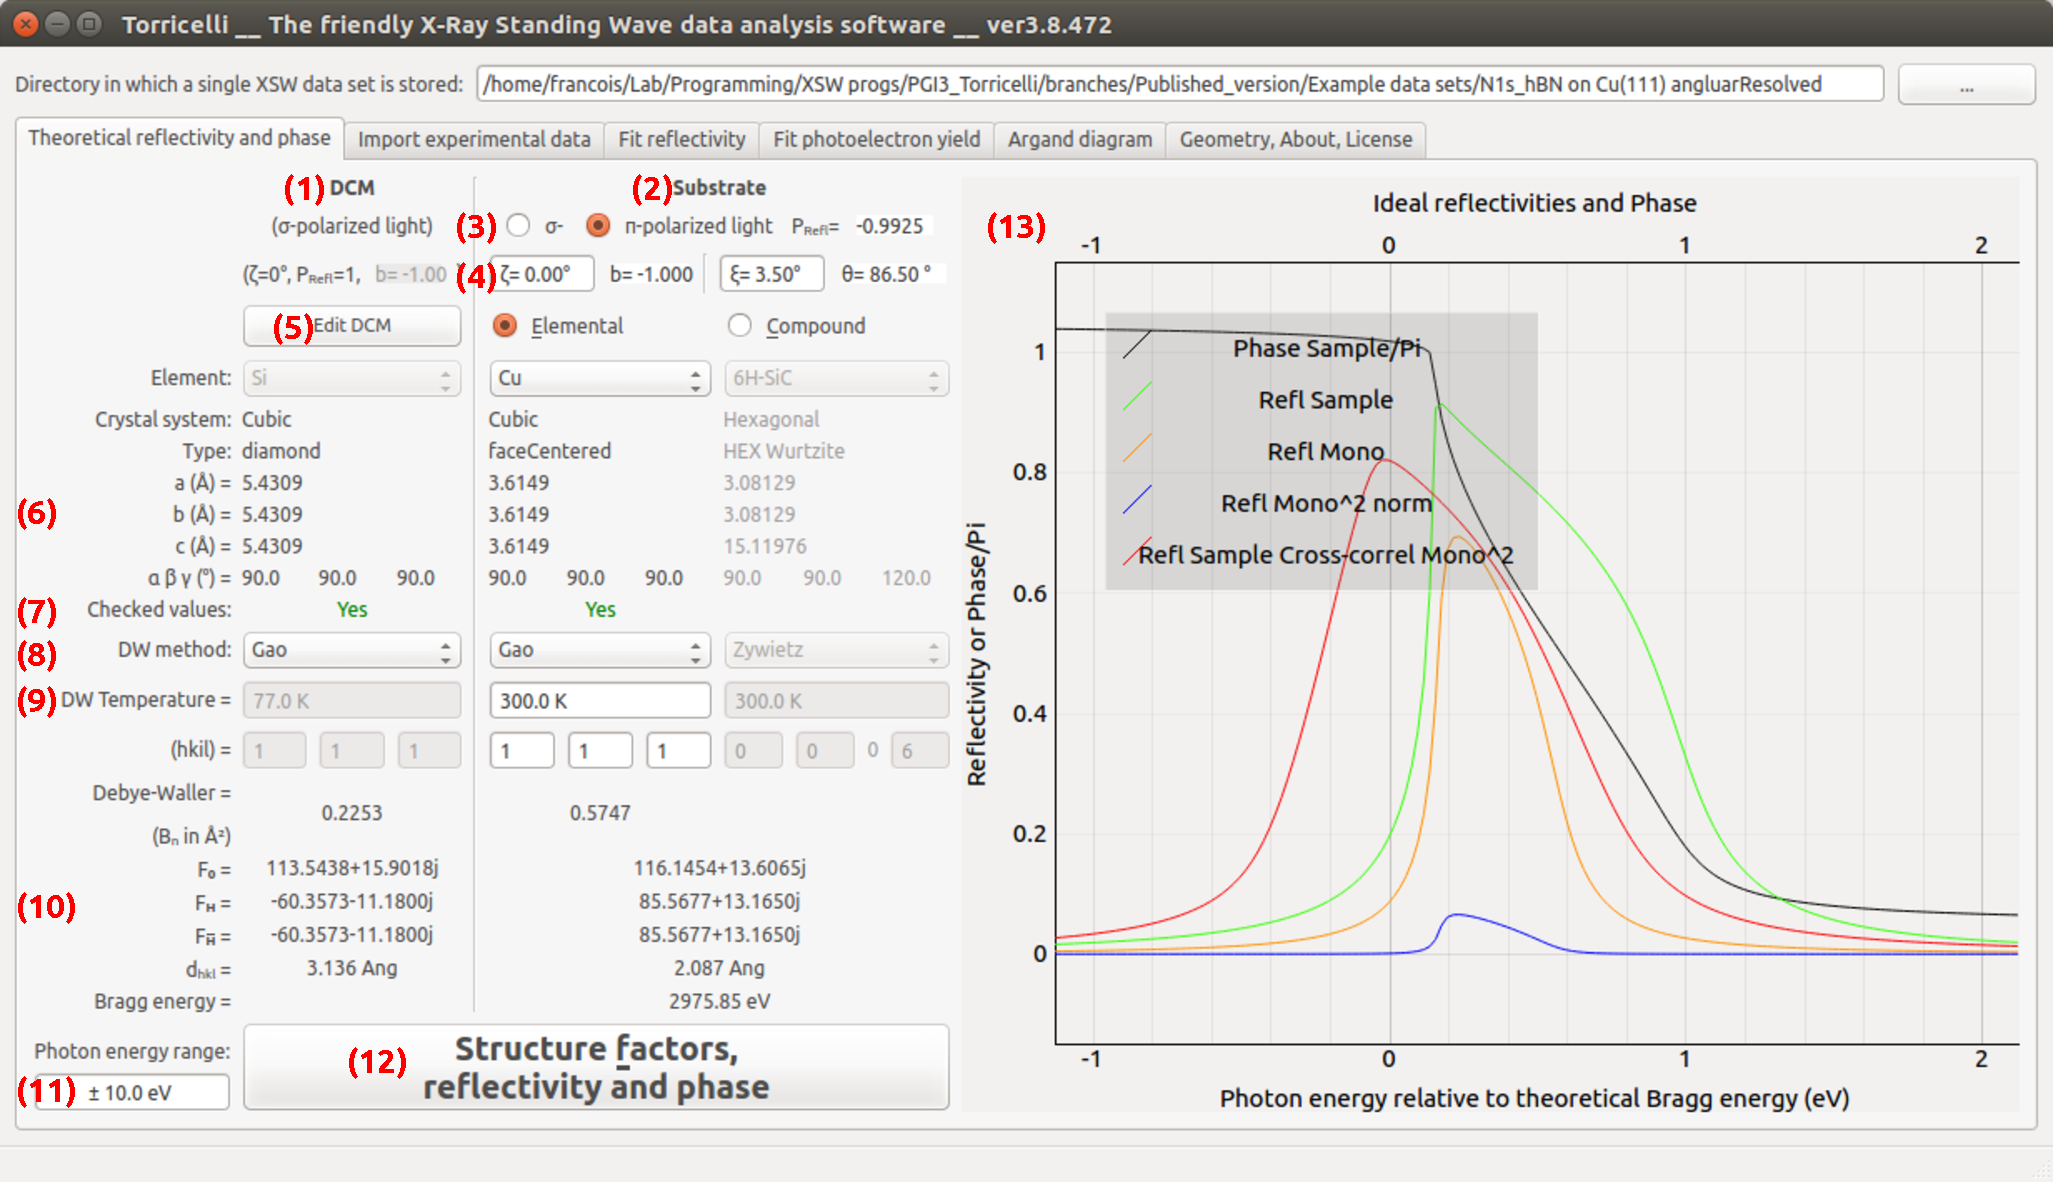
\includegraphics[width=1.2\textwidth]{img/Screenshot_StructureFactor.pdf}
  \caption{Screenshot of the \emph{Theoretical reflectivity and phase} tab of \textsc{Torricelli}.}
  \label{fig:structFac}
\end{figure}

In order to calculate structure factors necessary to simulate the theoretical reflectivity and phase, the following steps need to be taken. First define the photon energy range for which you wish to compute the theoretical curves (11) (see Fig.~\ref{fig:structFac}). This must be larger than the experimental range. Then one needs to specify the double crystal monochromator (DCM) (1) and sample (2) parameters. The two beam-lines on which we have some experience (I09 at the Diamond Light Source and ID32 at the ESRF) are both equipped with a Si(111) DCM. In order to correctly calculate a theoretical reflectivity curve corresponding to the experiments, \textsc{Torricelli} takes the DCM into account. Typically, Si crystals are cooled with liquid nitrogen and have a temperature of 77~K, and the (111) Bragg reflection is used. DCM parameters may be changed by clicking the \keys{Edit DCM} button (5). The light polarization is chosen in (3). Now one needs to set up the sample.
\begin{figure}[!t]
  \centering
  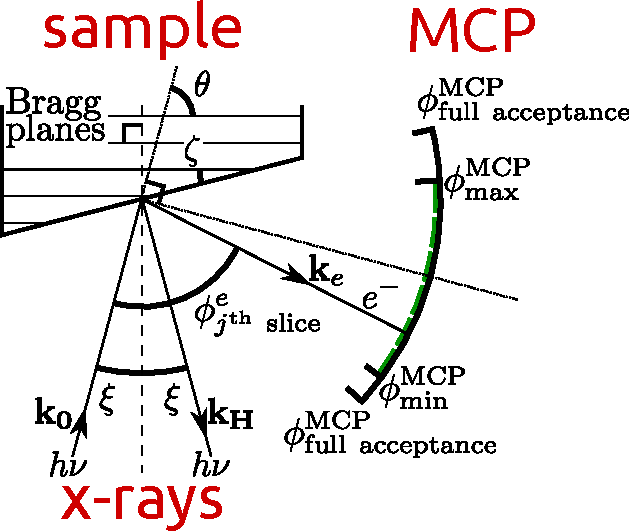
\includegraphics[width=.7\textwidth]{img/Geometry.pdf}
  \caption{Definition of all angles used by \textsc{Torricelli} ($\zeta$ and $\xi$ have positive values in the picture). This picture can also be found in the \emph{Geometry, About, License} tab  of \textsc{Torricelli}.}
  \label{fig:geometry}
\end{figure}
$\zeta$ (4) is the the angle between the sample surface and the Bragg planes. $\xi$ (4) is the deviation from perfect normal incidence on the Bragg planes ($\xi=3.5^\circ$ at the I09 beamline). See all angles depicted in Fig.~\ref{fig:geometry}. The parameters extracted from the database are displayed in (6). If those values were used in an actual XSW experiment, \textcolor{green}{Yes} will appear in (7). If \textcolor{red}{No}, please take the given values with care.

\parbox{0.9\linewidth}{\paragraph{Important} In the present state of the program, the \emph{DW Temperature} (9) only influences the calculation of the Debye-Waller factor. It does not affect the lattice parameter of your crystal. If you want to use a different crystal temperature, we advise to create a new line in the \fileTorri{imports/Databases/Lattices/CrystallographicData\_*.csv} file, use an explicit name, and adapt the lattice constant values.}\\\\

Once you defined the sample (2), the $hkl$ Miller indices of the wanted Bragg planes reflection (10) and the type of Debye-Waller factor (8), click on \keys{Structure factors, reflectivity and phase} (12) to first compute the structure factors. If the Bragg reflection is allowed, the structure factor values will be displayed (11) and the sample reflectivity $R^\mathrm{theo}_\mathrm{S}(h\nu)$, sample phase $\Phi^\mathrm{theo}_\mathrm{S}(h\nu)/\pi$, monochromator crystal reflectivity $R^\mathrm{theo}_\mathrm{M}(h\nu)$, the reflectivity of the double crystal monochromator $R^\mathrm{theo}_\mathrm{DCM}\left(h\nu\right) = \left(R^\mathrm{theo}_\mathrm{M}\right)^2\left(h\nu\right)$,  and cross-correlation between the sample reflectivity and the double crystal monochromator reflectivity $R^\mathrm{theo}_\mathrm{S+DCM}\left(h\nu\right) =  \left(R^\mathrm{theo}_\mathrm{S} \star \left(R^\mathrm{theo}_\mathrm{M}\right)^2_\mathrm{Norm}\right) \left(h\nu\right)$  will be computed and displayed in (13). Here and in the rest of the program, all curves are always shifted in photon energy such that 0~eV corresponds to the theoretical Bragg energy.


\paragraph{Note} From now on, \textsc{Torricelli} will remember the theoretical reflectivities and phases, and one does not need to redo this step unless \textsc{Torricelli} is restarted, or if data from a different sample are to be analyzed.

\paragraph{Auto-save} After clicking on (12), the structural factors are be saved in \dirData{results/Structure Factor.dat}, the, theoretical curves are saved in \dirData{results/Theoretical values.dat} and a screenshot of the plot is saved in \dirData{results/Theoretical values.png}. If these files already exist, they will be overwritten.


%%%%%%%%%%%%%%%%%%%%%%%%%%%%%%%%%%%%%%%%%%%%%%%%%%%%%%%%%%%%%%%%%%%%%%%%%%%
\chapter{Import experimental data} \label{chap:Import}
\paragraph{Note} For users of the I09 beam-line of the Diamond synchrotron, we advise to use the I09DataBrowser, a small software that converts the raw data to ASCII files ready to be used by CasaXPS and \textsc{Torricelli}. I09DataBrowser is developed and maintained by the \textsc{Torricelli} team.

In the following, the steps to be taken to import and normalize reflectivity and yield data are explained.

\begin{enumerate}
\item Choose the text files containing both the experimental reflectivity and $I^\mathrm{exp}_0$ (the intensity of the incident x-ray beam) (1) in Fig.~\ref{fig:import} and electron yield (2) curves (standard CasaXPS output), by clicking on the corresponding \keys{...} button (3). They should have the following formats:
  \begin{center}
    \fbox{\begin{minipage}{21em}
        \fileData{*.refl}:\\
        Contains the reflectivity and the beam intensity:
        \hline \\\vspace{10pt}
        Energy	I\_refl	I0\\
        2460.92	224.0	215042.0\\
        2460.99	225.0	214766.0\\
        2461.05	258.0	214328.0\\
        $\vdots$
    \end{minipage}}
  \end{center}
  \begin{center}
    \fbox{\begin{minipage}{33em}
        \fileData{*.txt} or \fileData{*.ey}: \\
        Contains the yield of each components as well as the standard deviations:
        \hline \\\vspace{10pt}
        Path of the file containing the full CasaXPS analysis (.vms)\\\\        
        Photon energy~	Reg\_Area(0) CPSeV~ StDev\_Reg\_Area CPSeV	$\cdots$\\
        2.460920e+003~	3.558958e+005~~~~~~~	8.186899e+002 $\cdots$\\
        2.460990e+003~	3.595590e+005~~~~~~~	7.855856e+002 $\cdots$\\
        2.461050e+003~	3.510015e+005~~~~~~~	7.930356e+002 $\cdots$\\
        $\vdots$
    \end{minipage}}
  \end{center}

\paragraph{Note} You can use the \keys{Display} buttons (4) to quickly check the content of a file, for instance, compatible number of points, or presence of some aberrant points (11-13). If you decide to remove some points from the data set, simply remove the corresponding lines \emph{in both files} using a text editor, and load again.
  \begin{figure}[!b]
  \centering
  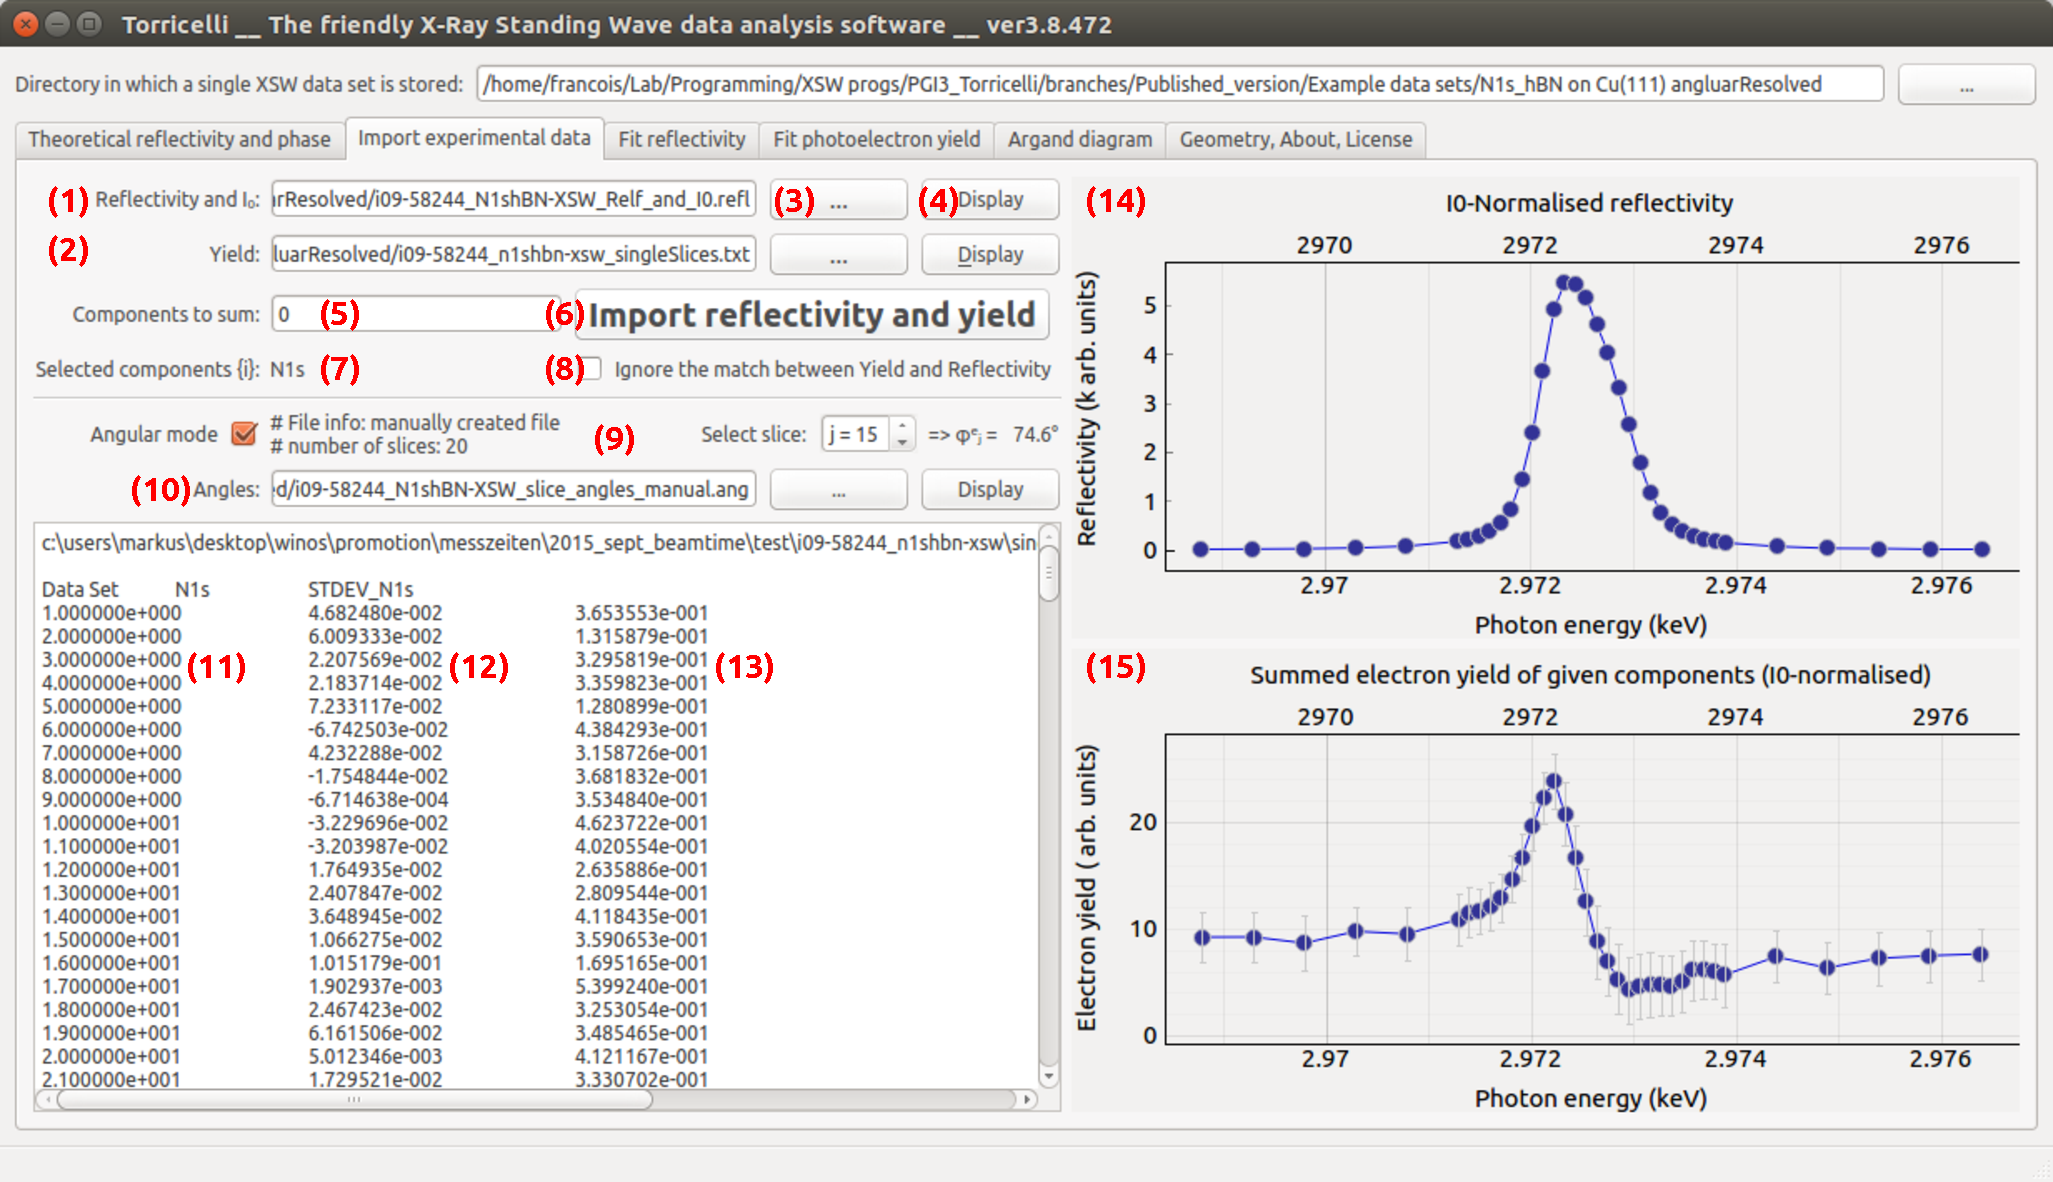
\includegraphics[width=1.2\textwidth]{img/Screenshot_Import.pdf}
  \caption{Screenshot of the \emph{Import experimental data} tab of \textsc{Torricelli}.}
  \label{fig:import}
  \end{figure}
  
\item Choose which component (5), or which set of components $\mathscr{S}$ you wish to analyze. In the field \texttt{Fit components} you can list the components numbers, separated by a space (e.g. '1' or '3 2 5'), that will be analyzed. Typically, a photoemission spectrum is fitted with one or more peaks, here also called components. If there is more than one, they will be summed. If nothing is given, the component 0 is the default. The component number start from 0 for the leftmost column, and it increments for columns going to the right. Every column with a component area (12) should be immediately followed by a column with the corresponding statistical errors (13).

\item By clicking on the \keys{Import reflectivity and yield} button (6), the data are normalized by $I^\mathrm{exp}_0$, and displayed (14 and 15). \textsc{Torricelli} will automatically check that both files have the same photon energies in the first column (111). If the photon energies are not defined as shown in the instance chosen for Fig.~\ref{fig:import}, this option can be removed by checking \texttt{Ignore the match between EY and Refl} (8). This check does not influence the data analysis, it only makes sure you are not mixing different data files. In angular mode, this check is not performed.

\item In the case of angular-resolved acquisition of photoelectrons, we recommend to save each angular-resolved data set (slice) sequentially in the yield file (for the same reflectivity file). It is then  possible to choose the slice number (9) to be analyzed by checking \texttt{Angular mode}. The corresponding $\phi_j^e$ must be given in the file \texttt{*.ang} file (10) so that it can be displayed in this tab, and also copied in the Fit Yield tab (See Fig.~\ref{fig:geometry}) in view of the calculation of the photoemission correction parameters.
    \begin{center}
    \fbox{\begin{minipage}{31.5em}
        \fileData{*.ang}: Contains the $\phi_j^e$ value corresponding to each slice $j$
        \hline \\\vspace{10pt}
        \# this file contains the angles corresponding to the centers of the slices\\
        \# File info: manually created file\\
        \# number of slices: 20\\
        \\
        slice	angle\\
        0~~~~	116.6\\
        1~~~~	113.8\\
        2~~~~	111.0\\
        3~~~~	108.2\\
        4~~~~	105.4\\
        5~~~~	102.6\\
        $\vdots$~~~~~~~~~$\vdots$
    \end{minipage}}
  \end{center}
In CasaXPS, you just have to put all spectra in the same folder before you load. The file name is used to order the files. Note that by simply scrolling on the slice number, the data are automatically imported (you do not need to press the button (6)).
  

\end{enumerate}

\paragraph{Note} If the working directory (see (1) in Fig.~\ref{fig:Tab}) is changed, \textsc{Torricelli} will try to find both the reflectivity, yield and angle files in this directory. They should have the extensions \texttt{.refl}, \texttt{.txt} or \texttt{.ey} and \texttt{.ang} respectively. If several files of the same type are present, the user has to choose the correct file manually.

\parbox{0.9\linewidth}{\paragraph{Important} \red{Do not forget that the definition of  $\phi_j^e$ includes $\xi$.}}


\parbox{0.9\linewidth}{\paragraph{Important} If you are using CasaXPS (or a similar program) to fit your spectra you have to pay attention to the statistical error calculation. CasaXPS uses the Monte Carlo method to fit the data \cite{Mercurio2013}. To estimate the statistical errors CasaXPS introduces a theoretical noise and assumes it to follow a Poisson distribution. This is a reasonable assumption for pulse counted data. However in modern detectors which rather use MCPs than channeltrons it can happen that your experimental noise is not Poisson distributed. In that case the statistical errors from the fits of your spectra will be wrongly estimated. To check in CasaXPS if your noise is Poisson distributed and to correct it, open a spectrum and fit a region on a flat area (just background intensity) of your spectrum using \texttt{regression} as background type. Than activate the display of the residuals. CasaXPS should show the \texttt{Residual STD} of your region fit. If your noise is Poisson distributed this value should be around $1$. If that is not the case there is an option for a correction. First select all your spectra. In the \texttt{Processing} window, go to the tab \texttt{Calculator} and press the button \keys{Poisson Adjust Selection}. When you now check the residual STD they should be around $1$. To have the option \texttt{Poisson Adjust} you have to use at least version \texttt{2.3.17 PR 1.1} of CasaXPS.}


  \paragraph{Auto-save} At this point nothing new is saved. 


%%%%%%%%%%%%%%%%%%%%%%%%%%%%%%%%%%%%%%%%%%%%%%%%%%%%%%%%%%%%%%%%%%%%%%%%%%%
\chapter{Fit reflectivity} \label{chap:FitRefl}
\begin{figure}[!b]
  \centering
  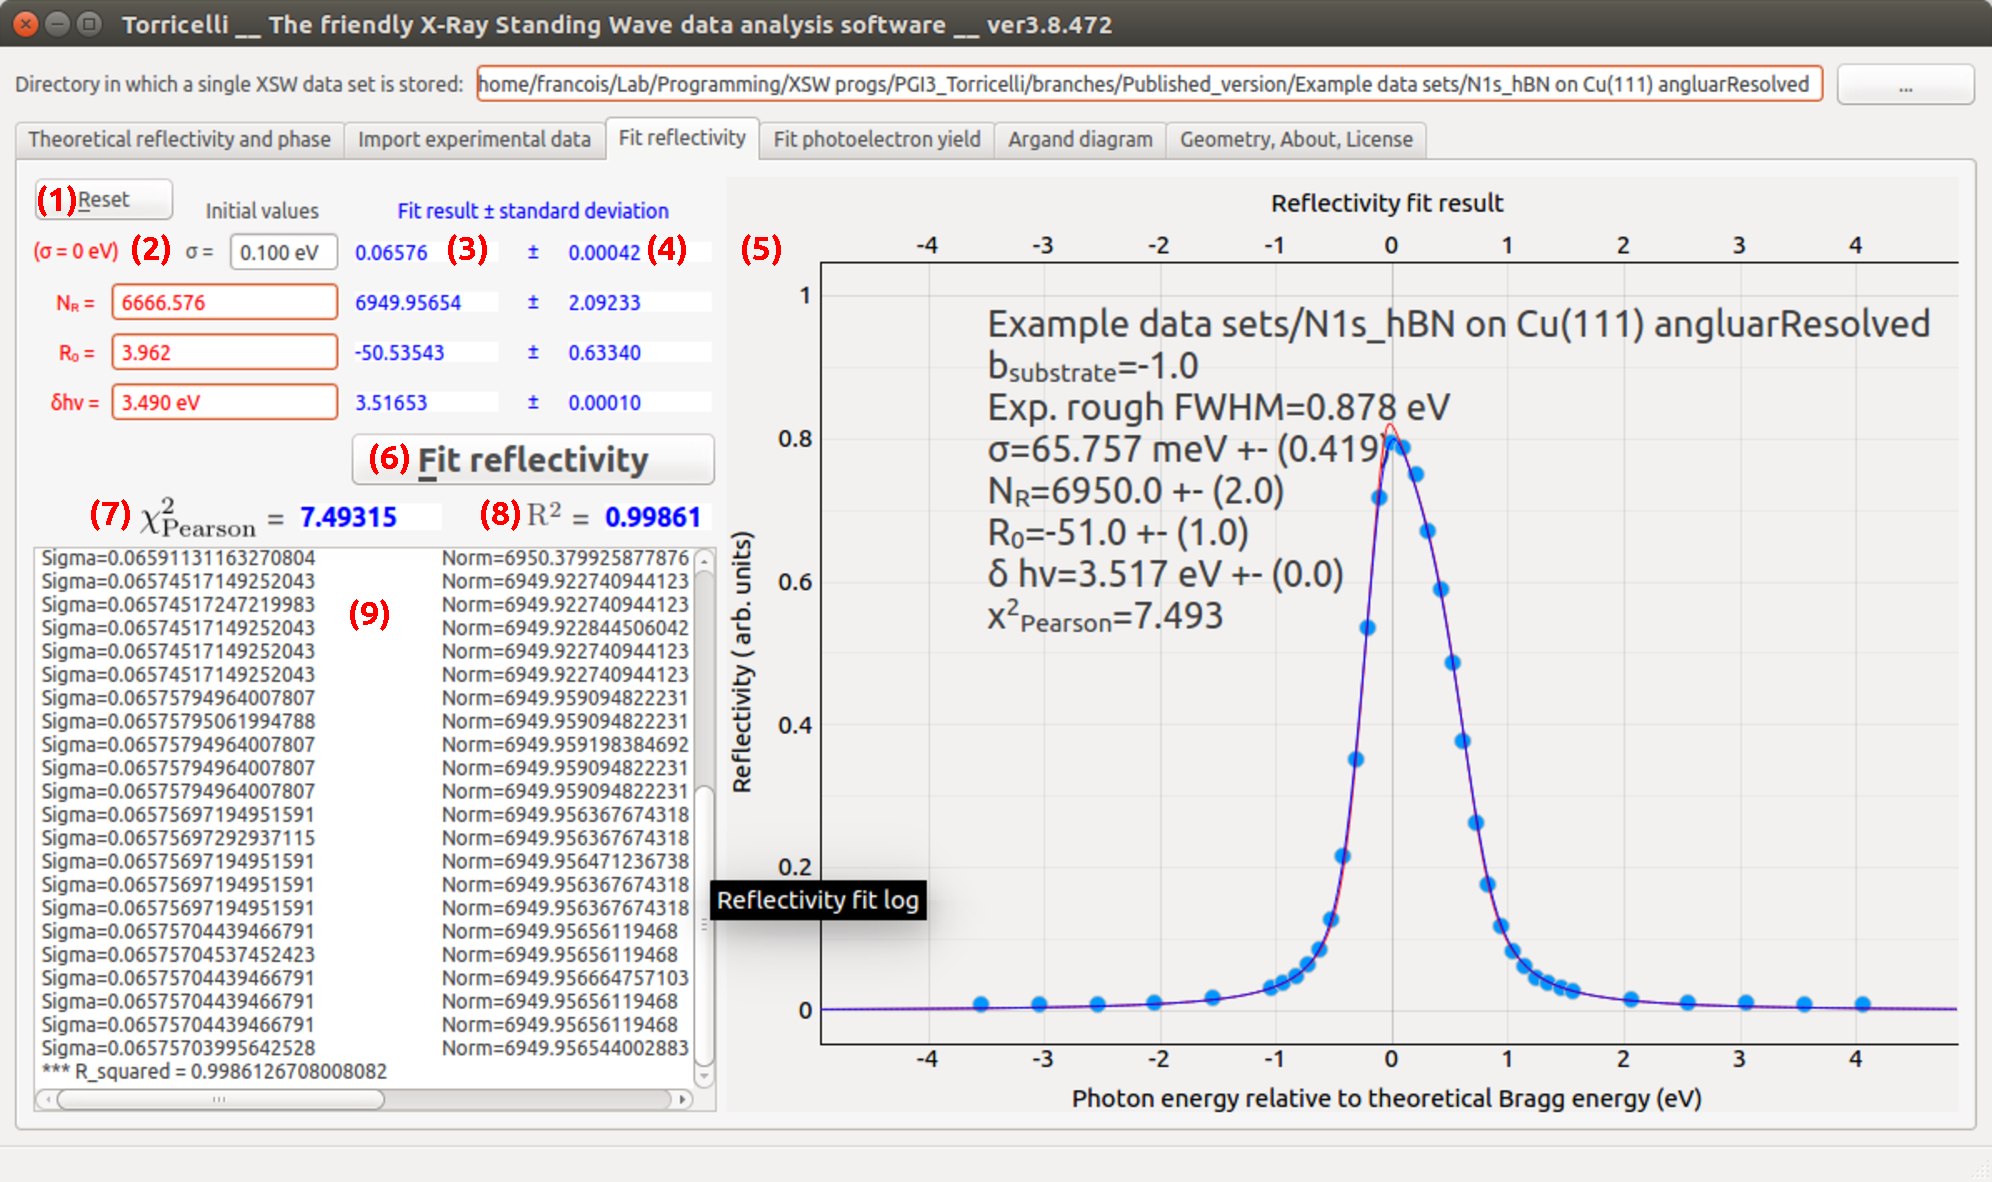
\includegraphics[width=1.2\textwidth]{img/Screenshot_FitRefl.pdf}
  \caption{Screenshot of the \emph{Fit reflectivity} tab of \textsc{Torricelli}.}
  \label{fig:refl}
\end{figure}

The fit is performed by minimizing
\begin{align} \label{eq:Refl}
  \mathcal{R}_R(\underline{\delta h\nu}, \underline{\sigma}, \underline{R_0}, \underline{N_R})  = \, R^\mathrm{model}\left(h\nu, \underline{\sigma}\right) - \frac{R^\mathrm{exp}(h\nu + \underline{\delta h\nu})-\underline{R_0}}{\underline{N_R}}
\end{align}
using the Levenberg-Marquardt method \cite{Levenberg1944,Marquardt1963,lmfit}. By default, the data points in the residuals are not weighted by a standard error because the later is not known. If one wishes to weight each reflectivity data point differently (e.g., if the standard errors are known), the code needs to be modified. The fitting parameters are: the background $\underline{R_0}$, the normalization $\underline{N_R}$, the photon energy shift $\underline{\delta h \nu}$ and the gaussian broadening $\underline{\sigma}$. The initial guess of $\underline{N_R}$ and $\underline{R_0}$ are such that the reflectivity difference between maximum and minimum as well as origin are the same between the data points and the theoretical curve. $\underline{\delta h \nu}$ is chosen such that the highest reflectivity point of the data and of the theoretical curve lie at the same photon energy. The default initial value of $\underline{\sigma}$ is 0.1. All initial values are displayed in red and fit results in blue.

\paragraph{Note} The lower the value $\sigma$, the better the crystal quality. The value of $\sigma$ for SiC is typically 0.05~eV, and for coinage metals 0.1-0.2~eV.


Press the \keys{Fit reflectivity} (6) button (see Fig.~\ref{fig:refl}). If the fit converges, the normalized experimental data together with the fitting theoretical curve are displayed as blue points and line (5), respectively. The experimental points correspond to the first term of Eq.~\ref{eq:Refl}. The red line corresponds to $R^\mathrm{theo}_\mathrm{S} \star \left(R^\mathrm{theo}_\mathrm{M}\right)^2_\mathrm{Norm}$, that is \emph{without} gaussian broadening ($\sigma=0$).

If the fit does not converge, you can try to modify the initial parameters (2) (e.g., increasing $\underline{\sigma}$ usually helps to find convergence, the other values are usually very good). The fit results are saved as text file and picture, see Chap.~\ref{chap:data folder}. It is possible to reset the initial values to the guess made by \textsc{Torricelli} by clicking on \keys{Reset} (1). 


In the absence of standard errors, the standard $\chi_\mathrm{red}^2$ is not defined. Therefore, the Pearson's chi-squared ($\chi_\mathrm{Pearson}^2$, see Eq.~1.8 in Ref.~\cite{GreenwoodBook}) and the coefficient of determination ($R^2$, see Sec.~1.3 and 11.2 in \cite{DrapperSmith}) are displayed (7, 8) in order to evaluate the quality of the fit \cite{GlantzSlinker, DrapperSmith} without the knowledge of the variance. They are defined as follows:
\begin{equation*}
\chi_\mathrm{Pearson}^2 \equiv \frac{1}{\mathcal{DF}}\sum_\mathrm{exp. h\nu} \frac{\Big(R^\mathrm{exp}(h\nu) - R^\mathrm{model}(h\nu)\Big)^2}{R^\mathrm{model}(h\nu)}
\end{equation*}
and
\begin{equation}
  R^2\equiv 1 - \frac{SS_\mathrm{res}}{SS_\mathrm{tot}},
\end{equation}
with $\mathcal{DF}$ the number of degree of freedom and
\begin{align}
  SS_\mathrm{res} &= \sum_\mathrm{exp.~h\nu} \left(R^\mathrm{exp} (h\nu) - R^\mathrm{model} (h\nu)\right)^2 \\
  SS_\mathrm{tot} &=\sum_\mathrm{exp.~h\nu} \left(R^\mathrm{exp} (h\nu) - \bar R^\mathrm{exp} \right)^2\\
  \bar R^\mathrm{exp}&=\frac{1}{n} \sum_\mathrm{exp.~h\nu}^n R^\mathrm{exp} (h\nu)
\end{align}
where the sums run over all experimental $h\nu$ values, and $n$ is the total the number of experimental points. $R^2$ values range from 0 (bad fit) to 1 (good fit).


\parbox{0.9\linewidth}{\paragraph{Important} If this fit is not good, it is of no use to continue the analysis! Check the parameters you used for the sample crystal.}


\paragraph{Auto-save} After clicking (6), the fit results are saved as ASCII file and pictures in \dirData{results/Exp\_refl\_norm\_centred.dat}, \dirData{results/Fit\_refl.log}, \dirData{results/Fit\_result\_refl.png} and \dirData{results/Fit\_result\_refl.dat}.



%%%%%%%%%%%%%%%%%%%%%%%%%%%%%%%%%%%%%%%%%%%%%%%%%%%%%%%%%%%%%%%%%%%%%%%%%%%
\chapter{Fit yield} \label{chap:FitYield}
\begin{figure}[!b]
  \centering
  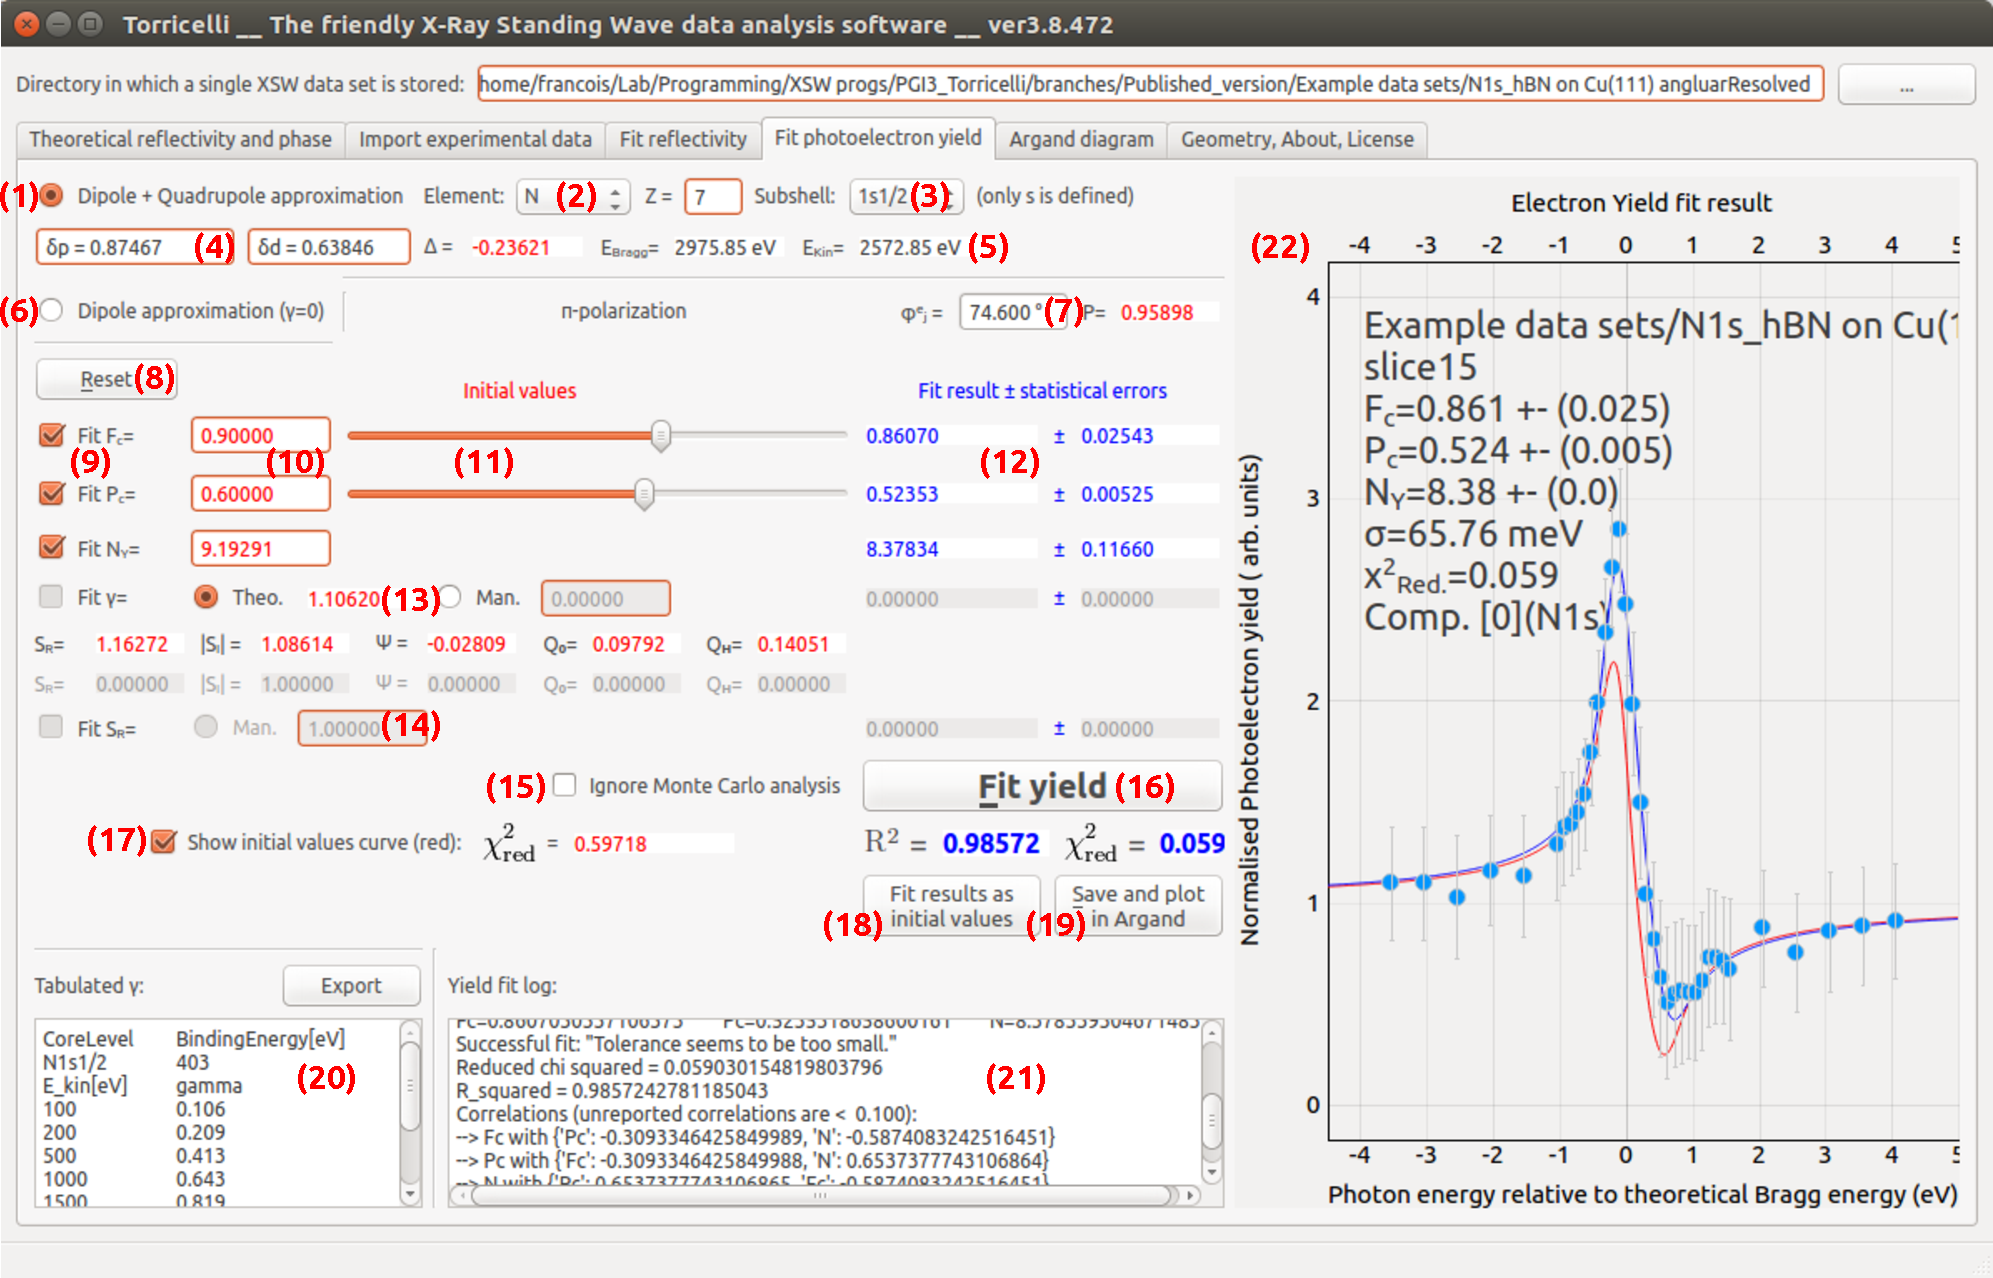
\includegraphics[width=1.2\textwidth]{img/Screenshot_FitYield.pdf}
  \caption{Screenshot of the \emph{Fit yield} tab of \textsc{Torricelli}.}
  \label{fig:yield}
\end{figure}

The fit is performed by minimizing
\begin{align} \label{eq:residual_Y}
  \mathcal{R}_Y(\underline{P_\mathrm{c}^\mathscr{S}}, \underline{F_\mathrm{c}^\mathscr{S}}, \underline{N_Y^\mathscr{S}})  = \, \bigg[Y^\mathrm{model}_\mathscr{S}& \left(h\nu, \underline{P_\mathrm{c}^\mathscr{S}}, \underline{F_\mathrm{c}^\mathscr{S}}, \underline{N_Y^\mathscr{S}}, \gamma, \phi\right) \nonumber \\
  & - \frac{Y^\mathrm{exp}_\mathscr{S}(h\nu+ \delta h\nu, \phi)}{\underline{N_Y^\mathscr{S}}}\bigg]\times\frac{\underline{N_Y^\mathscr{S}}}{\sigma_{Y^\mathrm{exp}_\mathscr{S}}(h\nu, \phi)}
\end{align}
using the Levenberg-Marquardt method. The values of $\delta h\nu$ and $\sigma$ are the result of the reflectivity fit and are fixed to fit the yield. In the simplest case, there are only three fitting parameters: the normalization factor $\underline{N_Y^\mathscr{S}}$, the coherent position $\underline{P_\mathrm{c}}$ and fraction $\underline{F_\mathrm{c}}$. If the statistical error $\sigma_{Y^\mathrm{exp}_\mathscr{S}}(h\nu, \phi)$ are not known or not reliable, it is possible to replace them by $\underline{N_Y^\mathscr{S}}$ in Eq.~\ref{eq:residual_Y} by checking \keys{Ignore Monte Carlo analysis} (15) (see Fig.~\ref{fig:yield}). It is possible to independently fix/fit each of the fit variables by un/checking them (9).

The level of approximation to be used to treat the photoemission process can be chosen: dipole (6) or dipole-quadrupole (1). Within the dipole-quadrupole approximation, $\Delta$  and the non-dipolar parameter $\gamma$ need to be calculated. To do so, the user must provide the element subject to photoemission (2) and the sub-shell under consideration (3). The corresponding photoelectron kinetic energy is then calculated and displayed $E_\mathrm{Kin}$ (5). This calculation ignores the sample work function. $E_\mathrm{Kin}$ is used to interpolate the $\gamma$ (13) value from the database \cite{Trzhaskovskaya2002a,Trzhaskovskaya2002b}, that is displayed in (20). Second, the value of $E_\mathrm{Kin}$ must then be given in the NIST Electron Elastic-Scattering Cross-Section Database version 3.2 (available on-line) to obtain $\delta p$ and $\delta d$ (4). A screenshot of the program \verb+Elastic32+ is given in Fig.~\ref{fig:NIST}. Afterwards, the user must copy the $\delta p$ and $\delta d$ in \textsc{Torricelli} so that $\Delta$ can be calculated. Finally, $\phi_j^\mathrm{e}$ (7) is used to calculate the polarization factor $P$ (in case of $\pi$-polarization). The value of $\phi_j^\mathrm{e}$ is automatically updated if an angle file is given in the import tab, if not this value must be given by hand. Once $\xi$, $\zeta$, $P$, $\gamma$ and $\Delta$ are known, \textsc{Torricelli} can calculate the photoemission correction parameter to the yield $S_R$, $S_I$ and $\psi$. Even within the dipole approximation, the $\phi_j^\mathrm{e}$ is needed (in case of $\pi$-polarization) to properly calculate $S_R$, $S_I$ and $\psi$. All initial values are displayed in red.
\begin{figure}[!b]
  \centering
  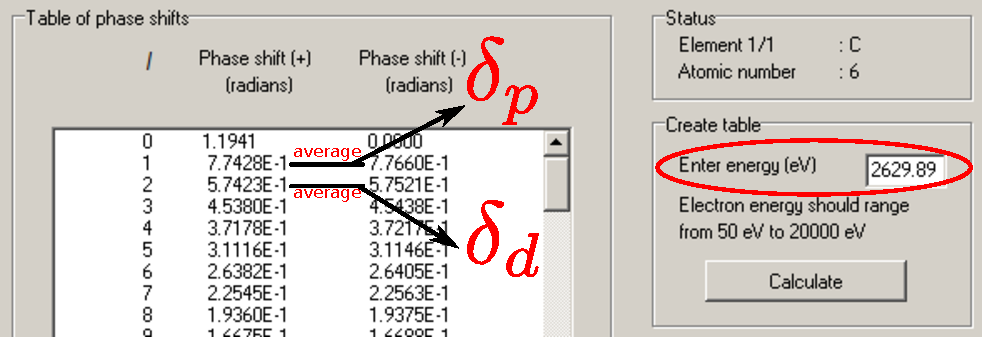
\includegraphics[width=.6\textwidth]{img/NIST.pdf}
  \caption{Screenshot of the Elastic32 program, the NIST Electron Elastic-Scattering Cross-Section Database to calculate $\delta p$ and $\delta d$ (Menu: Database/Phase shifts). Enter the adequate kinetic energy of the photoemitted electrons as calculated by \textsc{Torricelli}, and click \keys{Calculate}. }
  \label{fig:NIST}
\end{figure}

Press the \keys{Fit yield} button (16). If the fit converges, the normalized experimental data together with the fitting theoretical curve are displayed as blue points and line (22), respectively. The normalized statistical error are displayed as vertical red bars. Nonphysical negative or greater than unity $\underline{F_\mathrm{c}}$ or $\underline{P_\mathrm{c}}$ can still produce a very good fit. To overcome this, one has to set better initial values. After having fitted once, it is possible to display the theoretical curve with initial values in red (17). The initial values can be changed by typing the value (10), or by moving the cursor (11). The red curve in (22) will instantly update. Press the \keys{Fit yield} button (16) again once the initial values are set. The fit results together with their standard deviation (12) are displayed, as well as the coefficient of determination $R^2$ (see Chap.~\ref{chap:FitRefl}) and the $\chi_\mathr{red}^2$. Also, each step of the optimization are displayed in (21), as well as further fit results details. All fit result values are displayed in blue. It is possible to fit the $\underline{\gamma}$ (or $\underline{S_R}$) if your sample is completely disordered and you are confident to fix $F_\mathrm{c}$ to 0.

Once satisfied with the fit results, click on \keys{Save and plot in Argand} (19) to store the results (including the standard deviations and all other relevant parameters) in a list of all gathered results (See Chap.~\ref{chap:Argand}).


\paragraph{Note} The Monte-Carlo analysis in CasaXPS is usually slow. If you are in a hurry (during a beam-time), you may want to avoid this step and tell \textsc{Torricelli} not to read in the error bars and click \keys{Ignore Monte Carlo analysis} (15). This will remove the error bar weight on the data points, by effectively setting $\sigma_{Y^\mathrm{exp}_\mathscr{S}}(h\nu, \phi)=\underline{N_Y^\mathscr{S}}$. As a consequence, the error bars given by the fit procedure are not defined anymore and should not be used. Also, $\chi_\mathr{red}^2$ is not defined anymore.

\paragraph{Auto-save} In the \dirData{results} folder, pictures, normalized experimental data, fitted theoretical data as well as fit results are saved/updated automatically each time the \keys{Fit Yield} button is pressed. The created \texttt{RESULTS\_*.csv} file, that summarize the fit results and all used parameters, can be easily loaded by another program to consult the data.


%%%%%%%%%%%%%%%%%%%%%%%%%%%%%%%%%%%%%%%%%%%%%%%%%%%%%%%%%%%%%%%%%%%%%%%%%%%
\chapter{Argand diagram} \label{chap:Argand}
\begin{figure}[!b]
    \centering
    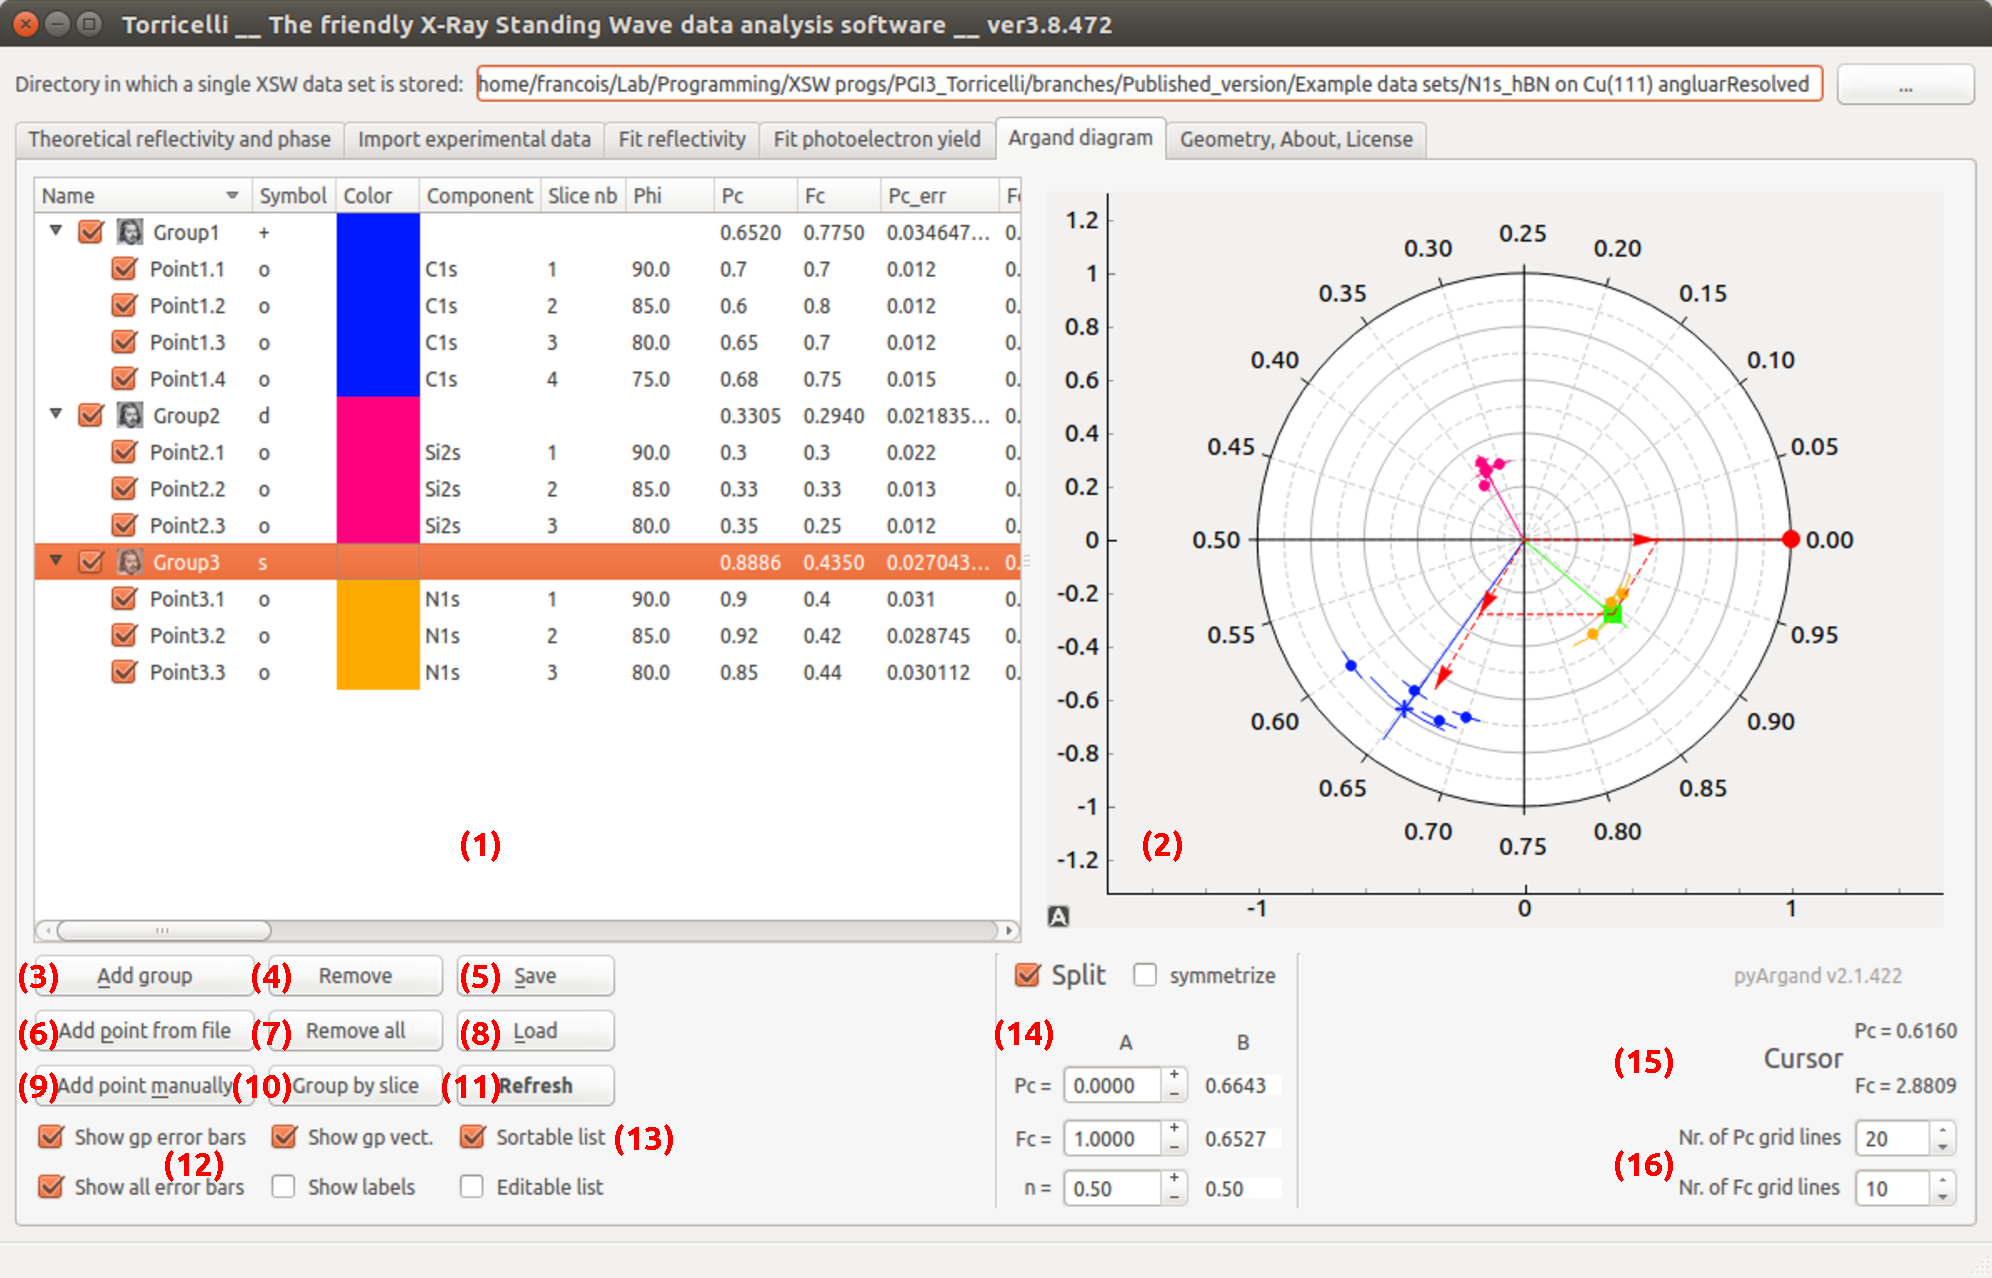
\includegraphics[width=1.2\textwidth]{img/Screenshot_Argand.pdf}
    \caption{Screenshot of the \emph{Argand diagram} tab of \textsc{Torricelli}.}
    \label{fig:Argand}
  \end{figure}
In this tab it is possible to display the fit results of the electron yield curve on an Argand diagram (2), a polar plot where each point is defined by a vector with angle $P_\mathrm{c}$ and length $F_\mathrm{c}$. The data are all listed in a list (1) and can be grouped (see Fig.~\ref{fig:Argand}). The vector average position and fraction of each group is automatically calculated and displayed (by default a + symbol and a line from the origin). One can display/hide independently every single data point (circle symbol by default, with the color of the group) or entire groups.  One can then move the data points from one group to another or within a group by a simple drag and drop. The selected point/s is/are highlighted in (2). Press \keys{Esc} to clear the selection. Points and groups can be removed by pressing \keys{Del} on the keyboard, or clicking the \keys{Remove} button in \textsc{Torricelli}. Double-click or \keys{F2} on any value-field permits to amend the values (only possible is \keys{Editable list} is selected). If several points are selected, a right-click on the name, color or symbol permit to apply the new property on the whole selection.

To add a group, just click on \keys{Add group} (3). To insert values in the selected group, one can either type-in the values manually (9), or choose the log file of a fit (6), or by clicking the \keys{Save and plot in Argand} button after having obtained a satisfying fit ((19) in the previous chapter). In the latter case, a new point is created in a group named like the working directory name. Furthermore, all relevant values are also saved and displayed in the list (1). The content of the list can be saved (5) in a text \verb+.csv+ file and reloaded at a later point (8). The format is chosen so that it can be easily loaded by another program (see Chap.~\ref{chap:data folder} for the content details). 

One can also decompose any data point $\mathscr{D}$ in the sum of two vectors ($\mathscr{A}$ and $\mathscr{B}$) (13). The $\mathscr{A}$ vector can be modified by moving it with the mouse (big red circle in (2)), or by typing values. The $\mathscr{B}$ will be updated automatically. $n$ corresponds to the respective amount of atoms populating each species. The \emph{Symmetrize} option forces $\mathscr{A}$ and $\mathscr{B}$ to have the same fraction.

By right-clicking in the diagram, one can export the picture by choosing 'Entire scene'. Several formats are possible, we advise though the \verb+.svg+ vector format which allows the easy modification of the picture with a dedicated program, like \textsc{Inkscape}. 

\paragraph{Auto-save} Additionally, the full content of the Argand diagram is  automatically saved regularly in the \fileData{autosave\_time\_description.csv} file in the working directory when the whole list is cleared, when the list is grouped by slices, after inserting a new point, or when \textsc{Torricelli} is closed. In each case, an explicit name is used.

The \fileData{results/RESULTS\_DataName\_TorricelliVersion.csv} file is created/updated each time the fit yield button is pressed in a given working directory. It summarizes all fit results obtained from a single data set for each $\mathscr{S}$ and each slice. If the fit button is pressed several times for the same  $\mathscr{S}$ and slice, only the last fit results are saved.



%%%%%%%%%%%%%%%%%%%%%%%%%%%%%%%%%%%%%%%%%%%%%%%%%%%%%%%%%%%%%%%%%%%%%%%%%%%
\chapter{Example data sets} \label{chap:Examples_Files}
In the directory \dirTorri{Examples data sets}, two data sets are given. In the following section, we give the fit results produced by \textsc{Torricelli} for a specific set of parameters.

\section{C1s\_H-QFMLG on SiC(0001)}
The first is a C 1s core level on quasifreestanding monolayer graphene on $6H$-SiC(0001), using the reflection (006). The data are angle integrated. Using $\pi$-polarization, $\zeta=0$, $\xi=3.5^\circ$, the Zywietz DW method, the core level component C1s\_QFMLG ($i=1$), $\phi_j^e=90^\circ$ and the dipole approximation, the reflectivity fit result gives $\sigma=45.7$~meV, $N_R=14396$, $R_0=154$ and $\delta h\nu = 2.67$~eV. The yield fit result provides $F_\mathrm{c}=0.871$, $P_\mathrm{c}=0.688$, $N_Y=128891.17$.

\section{N1s\_hBN on Cu(111) angluarResolved}
The second is a N 1s of hexagonal boron nitride monolayer grown on Cu(111) using the (111) reflection. The data are angle-resolved.  Using $\pi$-polarization, $\zeta=0$, $\xi=3.5^\circ$, the Gao DW method, the core level component N1s ($i=0$), the slice $j=15$, $\phi_j^e=74.6^\circ$ and the dipole-quadrupole approximation ($\delta p= 0.87467$, $\delta d=0.63846$, $\gamma=1.10620$), the reflectivity fit result gives $\sigma=65.8$~meV, $N_R=6950$, $R_0=-51$ and $\delta h\nu = 3.517$~eV. The yield fit result provides $F_\mathrm{c}=0.861$, $P_\mathrm{c}=0.524$, $N_Y=8.38$.

\chapter{Useful shortcuts} %%%*********************************%%%
\begin{itemize}
\item General ones:
  \begin{description}
  \item[\keys{Alt+F}]	 Presses the big button you always want to press on the active tab
  \item[\keys{Ctrl+PageDown}]	 Moves to the next tab
  \item[\keys{Ctrl+PageUp}]	 Moves to the previous tab
  \item[Mouse Wheel on tab] Scroll through tabs
  \end{description}
\item In graphical sub-windows:
  \begin{description}
  \item[Mouse wheel] zoom in/out
  \item[Left click + mouse move] x/y translation
  \item[Right click + mouse move] x/y re-scaling
  \item[Right click] menu with more options, including export options
  \end{description}
\item In the Argand list of group and points:
  \begin{description}
  \item[Double click on value] change the value in the selected field (Right-click is several items are selected)
  \item[\keys{F2} on value] change the value in the selected field
  \item[Double click on name] change the name. If several points are selected, a right-click will rename the selection with with increasing N: \texttt{name\_N}
  \item[\keys{Esc}] clear the item selection
  \end{description}
\end{itemize}


\chapter{The folder structure of \textsc{Torricelli}}
In the following we describe briefly all files present in the \textsc{Torricelli} program folder tree.

\dirtree{%
.1 \dirTorri{} \DTcomment{\textsc{Torricelli} home folder}.
.2 \file{Torricelli.py}\DTcomment{execute this file to start \textsc{Torricelli}}.
.2 \file{COPYRIGHT}\DTcomment{copy of the GNU General Public License v3}.
.2 \file{README}\DTcomment{Brief description of the files and folders}.
.2 \dird{Example data sets}.
.3 \file{ArgandTest.csv}\DTcomment{few ($F_\mathrm{c}$,$P_\mathrm{c}$) points for the Argand diagram}.
.3 \file{Argand\_BigFileTest.csv}\DTcomment{many ($F_\mathrm{c}$,$P_\mathrm{c}$) points for the Argand diagram}.
.3 \dirclosed{C1s\_H-QFMLG on SiC(0001)}.
%.4 \file{i09-22758\_C1sXSW\_Relf\_and\_I0.refl}\DTcomment{reflectivity, \emph{\textsc{Torricelli} input}}.
%.4 \dird{sum}.
%.5 \file{i09-22758\_C1sXSW\_allRegions\_\textbf{hnu}.dat}\DTcomment{core level measured with a photon energy of \textbf{hnu}}.
%.5 \file{i09-22758\_c1sxsw\_allregions\_2Comp\_ShirleyBgd.txt}\DTcomment{electron yield (CasaXPS analysis output), \emph{\textsc{Torricelli} input}}.
%.5 \file{i09-22758\_c1sxsw\_allregions\_2Comp\_ShirleyBgd.vms}\DTcomment{CasaXPS file}.
.3 \dirclosed{N1s\_hBN on Cu(111) angluarResolved}.
%.4 \file{i09-58244\_N1shBN-XSW\_Relf\_and\_I0.refl}\DTcomment{reflectivity, \emph{\textsc{Torricelli} input}}.
%.4 \file{i09-58244\_n1shbn-xsw\_singleSlices.txt}\DTcomment{electron yield (CasaXPS analysis output), \emph{\textsc{Torricelli} input}}.
.2 \dird{imports}.
.3 \file{user\_settings}\DTcomment{last settings used before closing \textsc{Torricelli}}.
.3 \file{GUI\_*}\DTcomment{gui modules}.
.3 \file{*.png and *.svg}\DTcomment{images}.
.3 \file{pyArgand.py}\DTcomment{Argand diagram library}.
.3 \dird{Databases}.
.4 \file{Database references.txt}\DTcomment{references for all files in the database}.
.4 \file{Nondipolar\_parameters\_of\_angular\_distribution\_Z1to100.ini}.
.4 \file{f0.csv}\DTcomment{f0 atomic scattering factor for all elements}.
.4 \dird{f1 and f2}\DTcomment{all f1 and f2 atomic scattering factor}.
.5 \file{si.nff}\DTcomment{f1 and f2 for Si}.
.4 \dirclosed{DW}\DTcomment{database necessary for the Debye-Waller factors}.
.4 \dird{Lattices}.
.5 \file{AtomCoordinates\_name-of-unit-cell.csv}\DTcomment{relative atomic position in this unit cell}.
.5 \file{CrystallographicData\_Compound.csv}\DTcomment{crystallographic parameters for compounds}.
.5 \file{CrystallographicData\_Elemental.csv}\DTcomment{crystallographic parameters for elemental crystals}.
}

\chapter{The folder structure of an analyzed data set} \label{chap:data folder}
Example of directory in which a single XSW data set is stored. In the folder \dir{sum} (depicted as \dirData{}), here chosen as working directory, the folder \dirData{results} will be created by \textsc{Torricelli} during the analysis.\\

\dirtree{%
  .1 \dird{C1s\_H-QFMLG on SiC(0001)}  \emph{or} \dirData{}.
  .2 \file{i09-22758\_C1sXSW\_Relf\_and\_I0.refl}\DTcomment{reflectivity, \emph{\textsc{Torricelli} input}}.
  .2 \file{i09-22758\_c1sxsw\_allregions\_2Comp\_ShirleyBgd.txt}\DTcomment{electron yield (CasaXPS analysis output), \emph{\textsc{Torricelli} input}}.
  .2 \file{autosave\_time\_description.csv}\DTcomment{Content of the Argand list automatically saved after pressing the \keys{Save and Plot in Argand} button}.
  .2 \dirclosed{slice1}\DTcomment{all data from the first angle-resolved data set}.
  .2 \dirclosed{slicen}\DTcomment{all data from the nth angle-resolved data set}.
  .2 \dird{sum}\DTcomment{all data from the sum of all angle-resolved data sets}.
  .3 \file{i09-22758\_C1sXSW\_allRegions\_\textbf{hnu}.dat}\DTcomment{core level measured with a photon energy of \textbf{hnu} (CasaXPS input)}.
  .3 \file{i09-22758\_c1sxsw\_allregions\_2Comp\_ShirleyBgd.vms}\DTcomment{CasaXPS analysis file}.
  .2 \dird{results}.
  .3 \file{Structure Factor.dat}\DTcomment{all structure factors}.
  .3 \file{Exp\_ey\_norm\_centred[0].dat}\DTcomment{electron yield of component 0 normalised to $I_0$ and relative to $E_\mathrm{Bragg}$}.
  .3 \file{Exp\_refl\_norm\_centred.dat}\DTcomment{reflectivity normalised to $I_0$ and relative to $E_\mathrm{Bragg}$}.
  .3 \file{Fit\_ey\_comp[0].dat}\DTcomment{best fit electron yield curve, component 0}.
  .3 \file{Fit\_ey\_comp[0].log}\DTcomment{log of the electron yield fitting}.
  .3 \file{Fit\_ey\_comp[0].png}\DTcomment{image from electron yield fit result}.
  .3 \file{Fit\_refl.log}\DTcomment{log of the reflectivity fitting}.
  .3 \file{Fit\_result\_refl.dat}\DTcomment{best fit reflectivity curve}.
  .3 \file{Fit\_result\_refl.png}\DTcomment{image from reflectivity fit result}.
  .3 \file{RESULTS\_C1s\_H-QFMLG on SiC(0001)\_Torricelli\_verx.x.x.csv}\DTcomment{list of results obtained from this working directory, updated after each click on \keys{Fit yield}}.
  .3 \file{Theoretical values.dat}\DTcomment{theoretical curves}.
  .3 \file{Theoretical values.png}\DTcomment{image of the theoretical curves}.
}\vspace{1cm}

Few \verb-.png- files simply record the graph displayed in \textsc{Torricelli}, for a quick printout. The \verb-.dat- files include actual data in ASCII that can be used in a scientific plotting program to produce high quality figures. The exact content of each of the \verb-.dat- is now detailed (for programmers, we also included the respective variable names.)
\begin{enumerate}
\item \file{\textbf{Theoretical values.dat}}
  \begin{itemize}
  \item[col1] Photon energy relative to the Bragg energy (\verb+self.Theory_photonEnergy+)
  \item[col2] Reflectivity of the sample crystal (\verb+self.Theory_Refl_sample+)
  \item[col3] Phase of the sample crystal (\verb+self.Theory_Phase_Sample+)
  \item[col4] Reflectivity of the monochromator crystal (\verb+self.Theory_Refl_Monochromator+)
  \item[col5] Phase of the monochromator crystal (\verb+self.Theory_Phase_Monochromator+)
  \item[col6] Final convoluted reflectivity of both crystal and monochromator (\verb+self.Theory_ReflSample_cc_ReflMono2+)
  \end{itemize}

\item \file{\textbf{Exp\_refl\_norm\_centred.dat}}
  \begin{itemize}
  \item[col1] Photon energy shifted by $\delta h \nu$ to fit the theoretical values\\(\verb!self.Exp_photonEnergy_BraggCentered +!$\delta h \nu$)
  \item[col2] Reflectivity normalized by $I_0^\mathrm{exp}$ for each photon energy, and multiplied by the average of all $I_0^\mathrm{exp}$, then shifted by $R_0$ and multiplied by $N_R$ to fit the theory ((\verb+self.Exp_Refl_Normalised -+ $R_0$)/$N_R$)
  \item[col3] Estimated statistical error on the reflectivity (square root of the previously normalized intensity) (\verb+self.Exp_Refl_Estimated_Error+/$N_R$)
  \end{itemize}

\item \file{\textbf{Fit\_result\_refl.dat}}
  \begin{itemize}
  \item[col1] Photon energy relative to the Bragg energy (\verb+self.Theory_photonEnergy+)
  \item[col2] Theoretical reflectivity curve best fit, including the gaussian broadening (\verb+bestFit_theo_refl+)
  \end{itemize}

\item \file{\textbf{Fit\_refl.log}} : List of all tested parameters configurations tested during the fitting procedure. The last one corresponds to the best fit.

\item \file{\textbf{Exp\_ey\_norm\_centred[$\mathscr{S}$].dat}}
  \begin{itemize}
  \item[col1] Photon energy shifted by $\delta h\nu$\\ (\verb-self.xsw_energies_BraggCentered- + $\delta h\nu$)
   \item[col2] Electron yield of the component set $\mathscr{S}$ provided (for example) by CasaXPS. It is normalized by $I_0^\mathrm{exp}$ for each photon energy, and multiplied by the average of all $I_0^\mathrm{exp}$ and divided by the $N_Y^\mathscr{S}$ (\verb+self.xsw_ey_normalised+/$N_Y^\mathscr{S}$)
     \item[col3] Statistical error of the electron yield of the component set $\mathscr{S}$ provided by CasaXPS normalized in the same way as the electron yield itself \\ (\verb!self.xsw_ey_error_casaXPS!/$N_Y^\mathscr{S}$)
	(NOTE that I09\_DataBrowser does not perform any normalisation)
  \end{itemize}

\item \file{\textbf{Fit\_ey\_comp[$\mathscr{S}$].dat}} :
  \begin{itemize}
  \item[col1] Photon energy relative to the Bragg energy (\verb!self.Theory_photonEnergy!)
  \item[col2] Electron yield best fit (\verb+self.Fit_Result_EY+)
  \end{itemize}

\item \file{\textbf{Fit\_ey\_comp[$\mathscr{S}$].log}} : List of all tested parameters configurations tested during the fitting procedure. The last one corresponds to the best fit. Each different value of the initial curve that is displayed will also be saved in this file.

\item \textbf{\texttt{*.csv} files}: Contains the fit results parameters separated by a comma. Each line correspond to a different data set. In the case of \verb+.csv+ file created by the Argand diagram tab, there is also a line corresponding to the average of all points contained in the group. The \file{autosave.csv} is rewritten each time the \keys{Save and plot in Argand} button is clicked and contains full content of the list visible in the Argand tab. The \file{RESULT\_*.csv} file is updated each time you click the \keys{Fit yield} button, and contains only fit results from the data present in the working directory. It remembers only the fit result of resulting from the last time you clicked \keys{Fit yield} for each set of component or angle chosen.

\end{enumerate}

\chapter{Miscellaneous}

\section{Reading or modifying the code}

Reading or modifying a function that is related to a specific object (Button, integer field, etc.)~in the graphical user interface works as follows. One opens the \verb2GUI_MainWindow.py2 file with the \texttt{QtDesigner} free software\footnote{\href{https://doc.qt.io/archives/qt-4.8/designer-manual.html}{https://doc.qt.io/archives/qt-4.8/designer-manual.html}} to obtain the object name. Then one can search the \texttt{Torricelli.py} file using a standard text editor to find which function is connected to this object. Both the command connecting an object to a function and the function itself are in the  \texttt{Torricelli.py} file.


\section{Few advices for efficiency} %%%*********************************%%%
\begin{itemize}
\item Use the shortcuts! Once you chose the working directory and set all your parameters/angles, you basically just have to press \keys{Alt+F} and \keys{Ctrl+PageDown} few times... And you are done!
\item Use the folder structure created by the DataBrowser (as explained in Chap.~\ref{chap:data folder}).
\item Save the electron yield file in the folder created by the DataBrowser, and use either a .txt or .ey extension.
\item Select the new folder for each new measurement (top of the window), then \textsc{Torricelli} will find all it needs automatically.
\item It is a good habit to keep an eye on the console window. Typically unexpected warnings or errors are displayed there.
\item It is an open source software: it can be modified but the modifications must maintain the same license.
\end{itemize}

\paragraph{Note}{Many file paths, folder paths and other settings are saved in the file \dirTorri{imports/user\_settings}. So when you close \textsc{Torricelli}, and open it again, the program is already pre-configured for you. }

%\section{Wish-list}
%\begin{itemize}
%\item Include temperature dependence of crystal parameters
%\item Port to \texttt{Python 3}
%\end{itemize}
%Do not hesitate to complete this wish list. Contact us!

%\section{Known bugs}
%\begin{itemize}
%\item Dragging the origin of the Argand diagram out of the field of view causes the Pc error bars to disappear. They come back if you move the plot in order to see the origin again.
%\end{itemize}



\begin{thebibliography}{99} % 99 is a rough guess of the total number of references
% \bibitem{} \myref{}{}{}{}{}{}{}
\bibitem{Bocquet2018} \myref{F. C. Bocquet, G. Mercurio, M. Franke, G. van Staaten, S. Wei{\ss}, S. Soubatch, C. Kumpf and F.S. Tautz}{\textsc{Torricelli}: A software to determine atomic spatial distributions from normal incidence x-ray standing wave data}{Computer Physics Communications}{235}{502}{2018}{10.1016/j.cpc.2018.06.009}

\bibitem{Mercurio2013} \myref{Mercurio, G. and Bauer, O. and Willenbockel, M. and Fairley, N. and Reckien, W. and Schmitz, C. H. and Fiedler, B. and Soubatch, S. and Bredow, T. and Sokolowski, M. and Tautz, F. S.} {Adsorption height determination of nonequivalent C and O species of PTCDA on Ag(110) using x-ray standing waves}{Phys. Rev. B}{87}{045421}{2013}{10.1103/PhysRevB.87.045421}

\bibitem{Levenberg1944} \myref{K. Levenberg}{A Method for the Solution of Certain Non-Linear Problems in Least Squares}{Quart. Appl. Math}{2}{164}{1944}{10.1090/qam/10666}

\bibitem{Marquardt1963} \myref{D. W. Marquardt}{An Algorithm for Least-Squares Estimation of Nonlinear Parameters}{J. Soc. Indust. Appl. Math.}{11}{431}{1963}{10.1137/0111030}

\bibitem{lmfit} \href{http://dx.doi.org/10.5281/zenodo.11813}{M. Newville, T. Stensitzki, D. B. Allen and A. Ingargiola -- \emph{\textsc{Lmfit}: Non-Linear Least-Square Minimization and Curve-Fitting for Python}.\\ Zenodo, (2014)}.

\bibitem{GlantzSlinker} A. Glantz and B. K. Slinker -- \emph{Primer of applied regression and analysis of variance}.\\ 2nd edition, McGraw-Hill (2001).

  \bibitem{GreenwoodBook} P. E. Greenwood and M. S. Nikulin -- \emph{A guide to chi-squared testing}.\\ John Wiley \& Sons (1996).
  
\bibitem{DrapperSmith} N. R. Draper and H. Smith -- \emph{Applied Regression Analysis}.\\ Wiley Series in Probability and Statistics, 3rd edition, Wiley-Interscience (1998).


\bibitem{Trzhaskovskaya2002a} \myref{M. B. Trzhaskovskaya, V. I. Nefedov, V. G. Yarzhemsky}{Photoelectron angular distribution parameters for elements Z=1 to Z=54 in the photoelectron energy range 100-5000~eV}{Atom. Data Nucl. Data Tables}{77}{97}{2001}{10.1006/adnd.2000.0849}

\bibitem{Trzhaskovskaya2002b} \myref{M. B. Trzhaskovskaya, V. I. Nefedov, V. G. Yarzhemsky}{Photoelectron angular distribution parameters for elements Z=55 to Z=100 in the photoelectron energy range 100-5000~eV}{Atom. Data Nucl. Data Tables}{82}{257}{2002}{10.1006/adnd.2002.0886}
\end{thebibliography}
\end{document}

